\documentclass[10pt,twocolumn,a4paper]{article}
\usepackage[margin=16mm,columnsep=5.5mm]{geometry}
\usepackage[T1]{fontenc}
\usepackage{newtxtext,newtxmath}
\usepackage{microtype}
\usepackage{amsmath}
\usepackage{graphicx}
\usepackage{booktabs}
\usepackage[numbers,sort&compress]{natbib}
\usepackage{stfloats}
\usepackage[hidelinks]{hyperref}

\graphicspath{{../results/}}
% Tighter space around floats, so three pages hold the tables, the figure and the bibliography.
\setlength{\textfloatsep}{6pt}
\setlength{\dblfloatsep}{6pt}
\setlength{\dbltextfloatsep}{6pt}
\setlength{\intextsep}{6pt}
\newcommand{\norm}[1]{\lVert #1 \rVert}
\newcommand{\lid}{\lambda_{\mathrm{id}}}

\title{Stable but Wrong: Fixed-Point Residuals as\\Reference-Free Reliability Signals for Image Restoration}
\author{Assaf Fleischer \quad Bar Milman \quad Michael Bazkor \quad Boaz Cohen  \quad Itay Shorian\\[2pt]
  \small Modern Computer Vision, Technion\\
  \small\url{https://github.com/milmanb/fixed-point-reliability}}
\date{}

\begin{document}
\maketitle

\begin{abstract}
Idempotent networks are trained so that $f(f(y)) = f(y)$, and recent work reads a small
idempotence residual as a sign of a reliable prediction. We test this reading on small Fashion-MNIST denoisers against the true
per-image error. The residual is zero for any exact projector, whatever
the error, and a first-order expansion shows that it probes the Jacobian along the model's own
displacement. For learned models it ranks errors within a corruption level (Spearman
$\rho = 0.70$ for a bottleneck autoencoder, 0.86 with skip connections). Yet each architecture has
an unseen corruption under which its outputs are stable but wrong and the residual misses them:
pixel masks for the bottleneck model, large box masks for the skip model. As a conformal error bar
the residual keeps its nominal 90\% coverage marginally, but covers only 61\% of pixel-mask images,
and calibrating on the training noise leaves 47\% coverage elsewhere. Deeper iterates rank worse;
cross-seed disagreement ranks better and is more robust to an idempotence penalty, yet inherits
both blind spots. A strong penalty makes the residual a worse signal ($\rho$ 0.62 and 0.63), and
without a warm-up both models collapse to constant images.
\end{abstract}

\section{Introduction}

Restoration networks are often applied where the clean image is unknown, and when they fail the
output can still look plausible, so a signal that flags unreliable outputs without ground truth
would be useful.

Idempotent Generative Networks (IGN)~\cite{shocher2024ign} train a network $f$ so that real data
are fixed points, $f(x) = x$, and other inputs land on that set, $f(f(y)) = f(y)$. Related
methods read the deviation from this property as a confidence
score~\cite{durasov2024zigzag,durasov2025it3,aljaff2025naign}. It is tempting to conclude that an
output which is a fixed point is also a correct one, but this does not hold in general: an exact
projector satisfies $P(P(y)) = P(y)$ for every input, including inputs it maps to a wrong
image. We ask how the residual behaves for learned models, which are only approximately
idempotent, and how training for idempotence changes it, in a controlled setting with known
errors. We find that (i)~the residual is a useful signal within a corruption
level, but each of two architectures has a corruption under which it misses the worst errors;
(ii)~a strong idempotence penalty makes the residual a worse signal, and without a warm-up it
collapses the model to a constant image; (iii)~as a conformal error bar the residual keeps its
marginal guarantee but breaks it badly on the corruption it is blind to, and neither deeper
iterates nor ensemble disagreement repair that gap.

\paragraph{Related work.}
Idempotence trains one-step generative
models~\cite{shocher2024ign,aljaff2025naign,zaman2025sign}; NAIGN~\cite{aljaff2025naign}
reads network drift as a distance to the data manifold. ZigZag~\cite{durasov2024zigzag} reports
per-sample correlations above 0.9 between a self-consistency residual and the loss;
IT$^3$~\cite{durasov2025it3} reports $-0.94$ between idempotence error and accuracy on ImageNet-C
per inference batch. Huang et al.~\cite{huang2023cycle} predict restoration uncertainty from
cycles that include $\norm{A_s f(y) - y}$; we test the residual itself and how idempotence training
changes it. We use SURE~\cite{stein1981sure,ramani2008mcsure} and split conformal
intervals~\cite{angelopoulos2021gentle}. Teneggi et al.~\cite{teneggi2023krcps} control risk
for diffusion sets, Everink et al.~\cite{everink2025surecp} calibrate imaging sets from
SURE, and Xu et al.~\cite{scrc2025} combine abstention with conformal sets. Hamidieh et
al.~\cite{hamidieh2026disagreement} argue that disagreement supplies the epistemic
uncertainty self-consistency misses.

\section{Method}

\paragraph{Setting.}
Let $x$ be a clean image and $y = A_s x + n$ an observation, with a known linear operator $A_s$ for
corruption $s$ and Gaussian noise $n$; a model $f$ must estimate $x$ without seeing it. A \emph{level} is one operator at one strength, and a \emph{family} groups the levels
of one operator. We use 13 levels in four families: Gaussian noise ($A_s = I$,
$\sigma \in \{0.1, 0.2, 0.3, 0.5\}$), Gaussian blur (width 0.5, 1, 1.5 or 2 pixels), pixel masks
(each pixel zeroed with probability 0.25, 0.5 or 0.75) and box masks (one random square of side 8
or 14). Blur and masks add weak noise ($\sigma = 0.02$), which the masks apply before zeroing.
Models are trained on Gaussian noise with $\sigma \le 0.25$ only, so $\sigma \ge 0.3$, blur and
masks are unseen.

\paragraph{Signals.}
With $|\Omega|$ the number of pixels, we compare
\begin{align*}
  g(y) &= \tfrac{1}{|\Omega|}\norm{f(f(y)) - f(y)}_1, & d(y) &= \tfrac{1}{|\Omega|}\norm{f(y) - y}_1,\\
  r_A(y) &= \tfrac{1}{|\Omega|}\norm{A_s f(y) - y}_1, & e(y) &= \tfrac{1}{|\Omega|}\norm{f(y) - x}_1.
\end{align*}
The residual $g$ and the displacement $d$ need only $f$ and $y$; $r_A$ also needs $A_s$ and equals
$d$ for denoising. For Gaussian noise we compute
$\mathrm{SURE}(y) = \tfrac{1}{|\Omega|}\norm{f(y)-y}_2^2 - \sigma^2
+ \tfrac{2\sigma^2}{|\Omega|}\operatorname{div} f(y)$ from four Rademacher probes and finite
differences ($\varepsilon = 10^{-3}$)~\cite{stein1981sure,ramani2008mcsure}.
Deeper iterates $g_k = \tfrac{1}{|\Omega|}\norm{f^{k+1}(y) - f^k(y)}_1$ and $q = g_2/g_1$ probe
further steps of the same map. Ensemble disagreement
$\mathrm{dis}(y) = \tfrac{1}{M|\Omega|}\sum_i \norm{f_i(y) - \bar f(y)}_1$ over $M = 3$ seeds
is their mean absolute deviation from the seed mean.

\paragraph{Why the residual can be blind.}
Write $\delta(y) = f(y) - y$ for the displacement. A first-order expansion of the second
application of $f$ gives
\begin{equation}
  g(y) = \tfrac{1}{|\Omega|}\norm{f(y + \delta) - f(y)}_1
       \approx \tfrac{1}{|\Omega|}\norm{J_f(y)\,\delta(y)}_1,
  \label{eq:taylor}
\end{equation}
so the residual probes the Jacobian along the one direction in which the model has just moved.
For an exact projector onto a smooth set, $\delta$ is normal to that set while $J_f$ projects onto
its tangent space, so $J_f\delta = 0$ whatever the error. A learned model can only be informative
where $J_f$ does not cancel its own displacement.

\paragraph{Models.}
The \emph{bottleneck} model is a convolutional autoencoder (602k parameters): three convolutions
(base width 32, SiLU, stride 2) down to $7\times7$, a 64-dimensional bottleneck, a mirrored decoder,
sigmoid output. The \emph{skip} model has the same convolutions with skip connections and no
bottleneck (230k parameters). We train on 55{,}000 Fashion-MNIST~\cite{xiao2017fashion} images
with $\sigma \sim \mathcal{U}[0.05, 0.25]$ for 15 epochs with Adam ($10^{-3}$, cosine decay, batch
256), minimizing
\begin{equation}
  \mathcal{L} = \norm{f(y) - x}_1 + \lid\,\norm{f(f(y)) - f(y)}_1,
  \label{eq:loss}
\end{equation}
averaged over pixels. Both models use $\lid \in \{0, 1\}$, the bottleneck also $\lid = 0.1$; three
seeds each. For $\lid > 0$ we ramp $\lid$ from 0 over five epochs; one run per model omits it.
Gradients normally flow through both applications of $f$; \emph{inner-only} training freezes the
outer $f$ in $f(f(y))$, as in IGN, and \emph{outer-only} freezes the inner output. Exact references:
projection onto a sphere around the training mean (radial) and onto the top 16, 64 or 256 principal
components (PCA).

\paragraph{Evaluation.}
On 10{,}000 test images we report Spearman's $\rho$ between a signal and $e$ within each level and
pooled over all levels, which corresponds to an unknown corruption, and the AUROC for detecting
the worst quartile of $e$. An image is \emph{flagged} when its signal is in the top quartile over
all levels, so a random score flags 25\% of any subset. Under masking the error grows with the
content of an image, so we add the brightness $b(y) = \operatorname{mean}(y)$ as a model-free
baseline and report partial correlations given $b$. For calibration we fit isotonic regression of
$e$ on a signal, per level or per family, on half the test images, score the other half, and
compare with a predictor that returns each level's mean error. Bootstrap 95\% intervals have a
half-width of about 0.01.

\paragraph{Coverage and selective risk.}
A ranking says nothing about how large the error may be. With $\hat u$ the isotonic fit of $e$ on
a signal over even-indexed test images, split conformal takes scores $e_i / \hat u(y_i)$, their
$\lceil (n{+}1)(1{-}\alpha)\rceil / n$ quantile $\hat q$, and reports
$\hat e_{\mathrm{hi}} = \hat q\,\hat u$ on the odd half, at $\alpha = 0.1$. Under exchangeability
this covers with probability $1-\alpha$~\cite{angelopoulos2021gentle}; what is informative is the
width and the coverage \emph{within} each family. We compare a marginal bound and a level-mean
bound, and a shift test (calibrate on the two training noise levels, deploy on the other eleven).
nAURC is the mean error of the accepted set when the highest-signal images are rejected first,
scaled so 0 is ranking by true error and 1 a constant score.

\section{Results}

  \begin{table*}[!t]
  \centering
  \scriptsize
  \caption{Error, residual and ranking quality. $e$ and $g$ are test-set means over levels and seeds.
    \emph{within}/\emph{noise}: Spearman $\rho$ with $e$, median over the 13 (or four noise) levels
    per seed, then mean over seeds. \emph{partial}: given brightness $b$. \emph{pooled} and
    \emph{AUROC}: all levels mixed. \emph{flagged}: share of worst-quartile mask errors whose $g$
    is in its top quartile over all levels (chance 25\%). $\mathrm{dis}$: disagreement of three
    seeds. Runs without a warm-up are constant maps.}
  \label{tab:main}
  \begin{tabular}{@{}lccccccccc@{}}
\toprule
& & & \multicolumn{3}{c}{$\rho(g, e)$} & $\rho(d, e)$ & $\rho(r_A, e)$ & $\rho(g, e)$ & \\
\cmidrule(lr){4-6}
training & $e$ & $g$ & within & noise & partial & within & within & pooled & flagged \\
\midrule
\multicolumn{10}{@{}l}{\emph{bottleneck model}} \\
none & 0.092 & 0.015 & 0.70 & 0.74 & 0.59 & 0.77 & 0.80 & 0.55 (0.46) & 18\% \\
$\lid =$ 0.1 & 0.092 & 0.013 & 0.71 & 0.73 & 0.56 & 0.77 & 0.80 & 0.52 (0.41) & 13\% \\
$\lid =$ 1 & 0.095 & 0.009 & 0.62 & 0.60 & 0.53 & 0.83 & 0.84 & 0.49 (0.34) & 10\% \\
$\lid =$ 1, inner only & 0.097 & 0.014 & 0.61 & 0.68 & 0.61 & 0.82 & 0.85 & 0.53 (0.46) & 22\% \\
$\lid =$ 1, no warm-up & 0.210 & 0.000 & -- & -- & -- & -- & -- & -- & -- \\
\multicolumn{10}{@{}l}{\emph{skip model}} \\
none & 0.086 & 0.019 & 0.86 & 0.92 & 0.48 & 0.49 & 0.72 & 0.52 (0.40) & 68\% \\
$\lid =$ 1 & 0.084 & 0.007 & 0.63 & 0.60 & 0.27 & 0.28 & 0.66 & 0.40 (0.33) & 31\% \\
$\lid =$ 1, no warm-up & 0.287 & 0.000 & -- & -- & -- & -- & -- & -- & -- \\
\bottomrule
\end{tabular}

\end{table*}

\begin{table}[t]
  \centering
  \small
  \caption{Conformal bounds at $\alpha = 0.1$ and selective risk, mean over three seeds. Pooled
    coverage is 0.90 in every row. \emph{width}: mean $\hat e_{\mathrm{hi}}$ for $g$ and for the
    level-mean bound. \emph{coverage}: of the $g$ bound on pixel/box masks, and after calibrating
    on the training noise levels (\emph{shift}). \emph{nAURC}: 0 = oracle, 1 = constant.}
  \label{tab:coverage}
  \setlength{\tabcolsep}{3.5pt}
\begin{tabular}{@{}lccccccc@{}}
\toprule
& \multicolumn{2}{c}{width} & \multicolumn{3}{c}{coverage, $g$} & \multicolumn{2}{c}{nAURC} \\
\cmidrule(lr){2-3} \cmidrule(lr){4-6} \cmidrule(l){7-8}
model & $g$ & level & pixel & box & shift & $g$ & $\mathrm{dis}$ \\
\midrule
bottleneck, $\lid{=}0$ & 0.174 & 0.138 & 0.61 & 0.96 & 0.48 & 0.41 & 0.48 \\
bottleneck, $\lid{=}1$ & 0.175 & 0.143 & 0.60 & 0.97 & 0.55 & 0.50 & 0.53 \\
skip, $\lid{=}0$ & 0.173 & 0.129 & 0.74 & 0.76 & 0.16 & 0.51 & 0.53 \\
skip, $\lid{=}1$ & 0.181 & 0.127 & 0.67 & 0.85 & 0.31 & 0.65 & 0.58 \\
\bottomrule
\end{tabular}

\end{table}

\subsection{Exact projectors}
For the radial and PCA projectors $g < 2\cdot10^{-15}$, and the right side of
Eq.~\eqref{eq:taylor} (radial and PCA-64 under noise) is at most $10^{-12}$, the round-off of the
finite differences, while the mean error lies between 0.04 and 0.23: the residual cannot rank
these errors at all. Deeper iterates change nothing, since $g_k \le \norm{J_f}^{k-1} g_1$.

\subsection{Learned models and their blind spots}
For the bottleneck model, $g$ ranks errors within a level with $\rho = 0.70$
(Table~\ref{tab:main}), and Eq.~\eqref{eq:taylor} holds in rank (Spearman 0.81 to 0.97 between
$g$ and its linearization for $\sigma \le 0.3$). Under noise the residual holds up as the noise grows
(0.75 at $\sigma = 0.1$, 0.72 at 0.5), while $d$ falls from 0.93 to 0.28 and SURE from 0.91 to 0.40.
The skip model's residual ranks better at 11 of the 13 levels, and its partial $\rho$ is higher at
the same 11 for every seed; its median is lower only because of the box masks. Brightness alone
reaches a median within-level $\rho$ of 0.51 to 0.55, and 0.96 under pixel masks, so raw scores
under masks and blur overstate the signals.

Pooled over all levels, $g$ reaches $\rho = 0.55$ and an AUROC of 0.69 for the bottleneck model,
against 0.12 for $d$ and 0.02 for $r_A$. The pooled score hides a blind spot
(Fig.~\ref{fig:failures}). Under 75\% pixel masks the bottleneck model's mean error is 0.234, five
times that at $\sigma = 0.1$, while its mean residual barely moves (0.014 against 0.011): it turns
sparse dots into a dim garment and treats it as a fixed point. Pixel masks hold 60\% of the
worst-quartile errors, and $g$ flags 18\% of them. The skip model has the opposite blind spot:
under box masks its within-level $\rho$ drops to 0.29 and 0.12, it flags under 1\% of the worst
box-mask errors, and 83--87\% of its top-10\%-error, below-median-$g$ images are large boxes.

\begin{figure}[t]
  \centering
  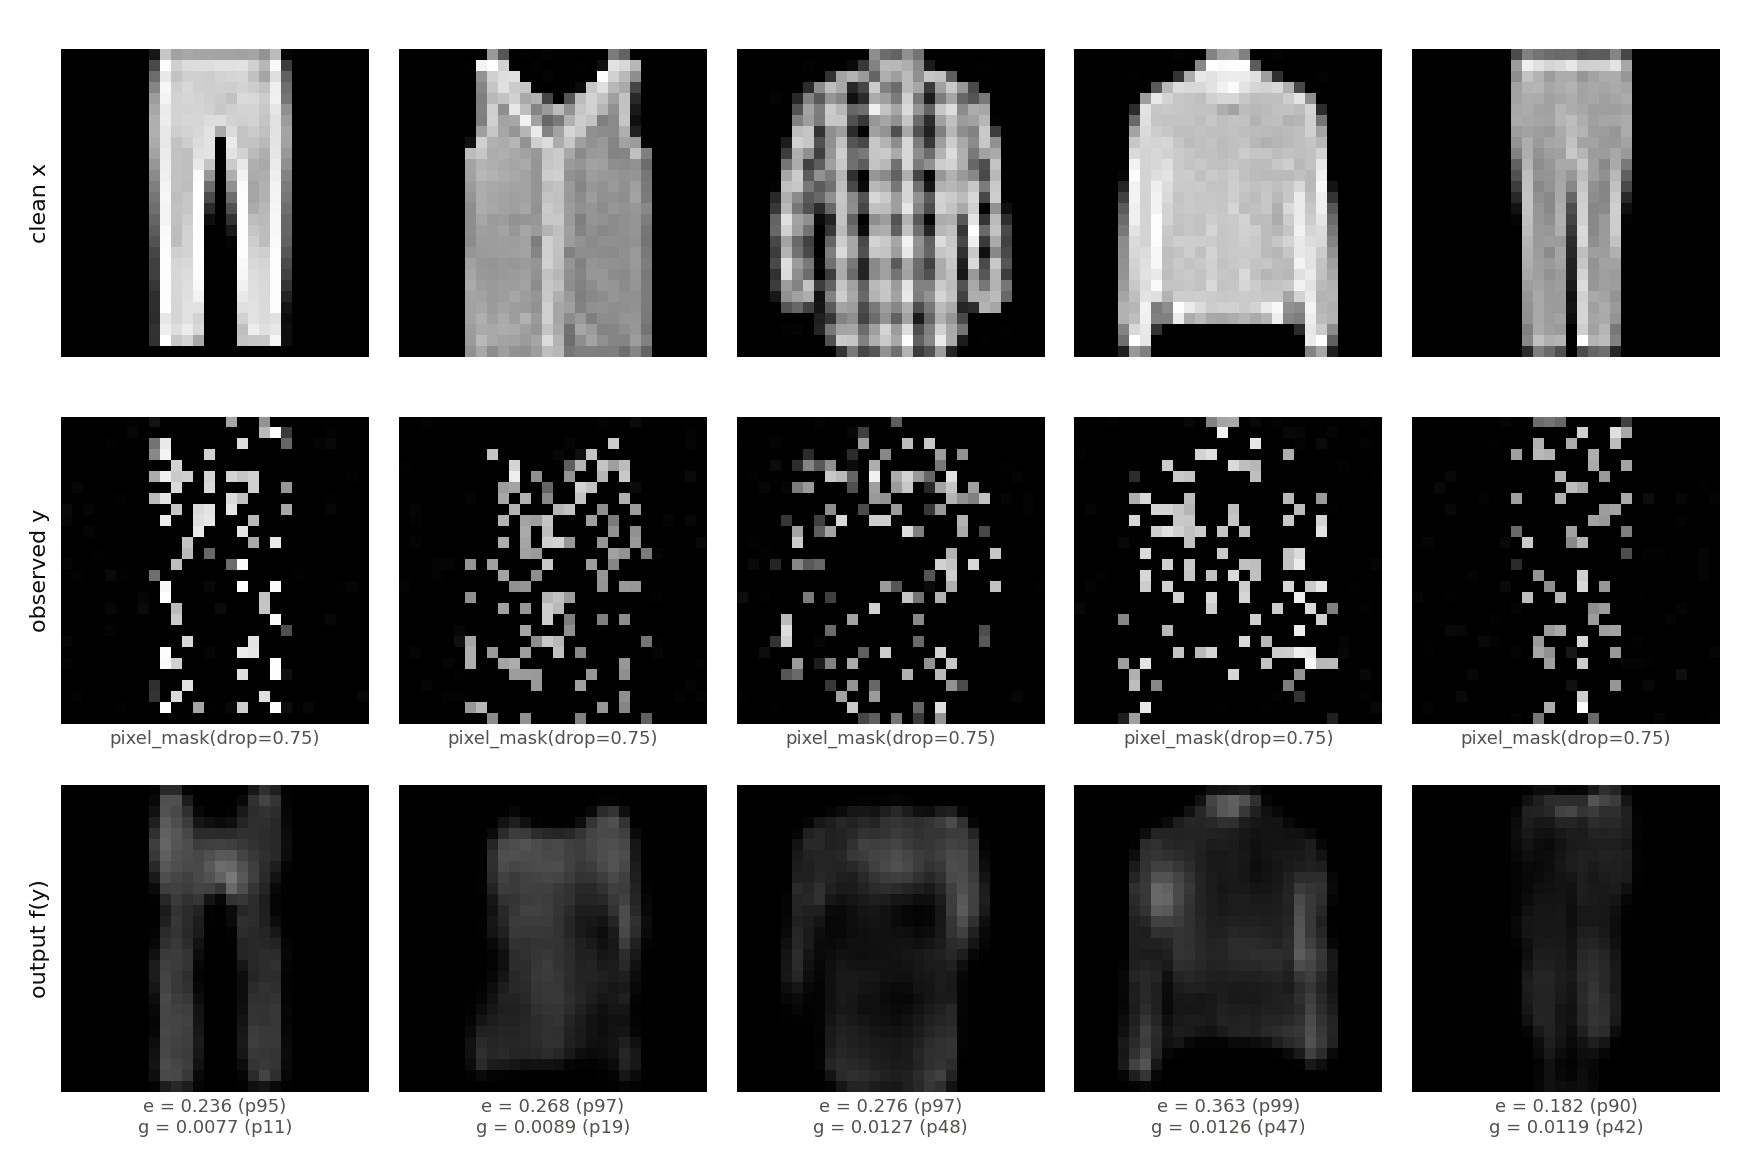
\includegraphics[width=0.98\columnwidth]{models/figures/failures_compact_dae_lam0_seed0.png}
  \caption{Stable but wrong: top-10\% error and below-median $g$ (bottleneck, $\lid = 0$, seed 0).
    98\% of such images are pixel masks.}
  \label{fig:failures}
\end{figure}

\subsection{Training for idempotence}
\label{sec:idem}
Without a warm-up, $\lid = 1$ collapses both architectures within one epoch to a constant image:
the bottleneck model to the per-pixel median training image (validation error 0.2106, residual
$10^{-6}$), the skip model to black (0.2885, residual $10^{-10}$). These losses, 0.21 and 0.29, are
far above the $\lid = 0$ solutions, so they are failures of optimization; the skip model is not
near-constant at initialization (output spread $8\cdot10^{-3}$ against $5\cdot10^{-6}$).

With the warm-up, mean error changes little (0.092 to 0.095; 0.086 to 0.084) but the residual falls
by 40\% and 61\% and becomes a worse signal: within-level $\rho$ falls from 0.70 to 0.62 and from
0.86 to 0.63, with no overlap between seeds. A weight of 0.1 leaves the within-level $\rho$
unchanged (0.71). All three routings lower it (0.62; 0.61 inner-only; 0.65 outer-only), but only
routes reaching the outer application also lose partial $\rho$, pooled $\rho$ and the pixel-mask
flagged share; they shrink $g$ by 26\% against 6\%.

\subsection{Calibration, coverage and selective risk}
\label{sec:coverage}
Each signal has a different scale in each family. After per-level calibration, pooled $\rho$ is
0.89 for $g$, 0.93 for $d$ and 0.94 for $r_A$ in the bottleneck model (0.92--0.93 skip); the
level-mean predictor already reaches 0.77 and 0.84. When only the family is known, $g$ is the best
calibrated signal (0.84 and 0.79).

The conformal bound on $g$ meets its nominal 90\% marginally and is narrower than a bound that
ignores the signal (0.174 against 0.183), but the level-mean bound is narrower still (0.137). By
family it covers 1.00 of noise and blur but only 0.61 of pixel masks (bottleneck) and 0.76 of box
masks (skip) --- Table~\ref{tab:coverage}. Under the shift test, coverage falls to 0.47 ($g$) and
0.19 ($d$, $r_A$) for the bottleneck model, and to 0.16--0.31 for the skip model. Deeper iterates
rank worse ($g_2$ 0.63, $g_3$ 0.60 against 0.70) with unchanged coverage; $q$ is uninformative
($\rho = 0.02$). Eq.~\eqref{eq:taylor} predicts this.

Ensemble disagreement ranks better within a level ($\rho = 0.79$ against 0.70; 0.76 against 0.62 at
$\lid = 1$; skip: 0.88 against 0.63 at $\lid = 1$). Where $g$ loses 0.09 and 0.24 under the
penalty, disagreement loses 0.03 and gains 0.04. It still inherits both blind spots: 0.59 coverage
and 20\% flagged on pixel masks, 1.2\% flagged on skip box masks. Three seeds of one architecture
fail the same way on an unseen operator. Rejecting the 20\% of images with
the largest $g$ lowers mean error from 0.092 to 0.084 (oracle 0.064; nAURC 0.41); $r_A$ and
brightness are worse than rejecting nothing. SURE self-calibration over-covers on noise (0.94).

\section{Discussion}
In our setting, a small idempotence residual is weak evidence of a correct restoration. For a
projector it carries no information. For the two learned models it is a useful signal within a
level, but each produces stable but wrong outputs under at least one unseen corruption, and the
residual misses most of them. Which corruption this is depends on the architecture.

Conformal calibration makes that a cost: the quoted guarantee is marginal and holds, while coverage
on the family the model is blind to fails with no warning~\cite{angelopoulos2021gentle}. A residual
is safe only over a corruption it was calibrated on. With $\lid = 1$ the residual became a worse
signal while restoration held; a diagnostic that is also a loss can lose information, here via
gradients through the outer application. Methods that minimize the residual at test
time~\cite{durasov2025it3} may face the same issue; we did not test this. Ensemble disagreement is
the better choice for such models, but it agrees with itself where it is wrong.

\tiny
\bibliographystyle{abbrv}  % ignores url/doi fields
\setlength{\bibsep}{0pt}
\bibliography{references}

\end{document}
